\documentclass{ctexart}

% Language setting
% Replace `english' with e.g. `spanish' to change the document language
\usepackage[english]{babel}

% Set page size and margins
% Replace `letterpaper' with `a4paper' for UK/EU standard size
\usepackage[letterpaper,top=2cm,bottom=2cm,left=3cm,right=3cm,marginparwidth=1.75cm]{geometry}

% Useful packages
\usepackage{amsmath}
\usepackage{graphicx}
\usepackage[colorlinks=true, allcolors=blue]{hyperref}

\title{中国科学技术大学交流生生存指北}
\author{ }
\date{ }

\begin{document}
\maketitle

\section{前言}
同学,当你看到这份生存指北的时候,首先恭喜你,你已经经过学校的重重选拔,即将作为一名交流生踏入中国科学技术大学的校园.相信你现在的内心一定是充满激动和喜悦的,一定是憧憬着在中国科学技术大学的交流生活的。这份生存指北将为你未来的生活提供参考.
\par 中国科学技术大学始建于1958年,后因文化大革命南迁至安徽合肥,秉持着{\bf{\textcolor{red}{红专并进,理实交融}}}的校训,迎着永恒的东风,已经走过66年(截止到2024年),学校设有32个学院,本科专业41个,含8个科教融合学院,是一所传统的理科强校

\section{前置技能学习}
在开始激动人心的交流生活前,请先了解以下知识:
\subsection{数学技能}
\subsubsection{数学分析}
请确保你没有忘记基本的积分技巧与常用积分公式,以及极限,级数等相关知识
%%TODO:这一部分请数学系的同学帮忙整理相关概念
\subsubsection{线性代数}
请确保你没有忘记线性代数的基本概念:
%%TODO:这一部分请数学系的同学帮忙整理相关概念
\subsection{计算机相关技能}
\subsubsection{科学上网}
鉴于有些资料在外网上比较丰富,所以建议大家学习如何用V2rayN和Clash.机场(可以提供上外网的节点,会收取一定的费用),这里推荐一个我自己用的机场\href{https://la.gsoula.life/}{高斯云}
\subsubsection{搜索引擎}
停止适用百度,试着使用必应,google(需科学上网)等搜索引擎
\subsubsection{AI}
ai是提高生产力的好帮手,学会正确使用ai是一件非常有必要的事情,下面介绍几个LLM
\begin{enumerate}
    \item ChatGPT:作为最早也是最先进的大语言模型,ChatGPT的数学能力和信息检索分析能力可以说是非常强大,因此对于一些数学问题或者比较简单的专业问题可以向GPT提问,但是注意甄别回答的正确性,因为不保证ai的回答是完全正确的,所以请结合自己的专业知识和搜索引擎进行甄别。需要注意的是,因为openai官方ban掉了中国信用卡,所以不能在openai官网上使用需要付费的GPT版本,一个好的解决办法就是使用中转站去使用ChatGPT,这里附一个我常用的中转站\href{https://api.bltcy.ai/}{柏拉图API},这个中转站不仅有ChatGPT还有其他大模型例如:suno,Midjourney等等
    \item Gemini:作为Google自研的多模态大模型,对图像和语言的处理和转换是做的相当好的,有兴趣的同学可以去\href{https://gemini.google.com/app?hl=zh-cn}{Gemini官网}体验一下%%OPT:有了解的同学可以补充说明一下
    \item Kimi:作为国产的ai,能很好的总结所给文章的大致内容,是阅读论文的好帮手,但是相应的,这个模型的数学能力较差,官网链接:\href{https://kimi.moonshot.cn/}{kimi}
\end{enumerate}
\par 使用大模型的时候还要学会正确地提prompt(关键词),prompt越准确,ai回答的越精准,具体提法可以参考这篇文章\href{https://zhuanlan.zhihu.com/p/660369244}{编写高质量Prompt的14个有效方法
}
\subsubsection{文档标记语言}
\begin{itemize}
    \item Q:什么是文档标记语言
    \item A:文档标记语言即在电脑上写文档所用的语言,类似于word但是更便于排版和输入公式,目前常用的有latex和markdown
    \item Q:为什么要使用文档标记语言
    \item A:在中国科学技术大学很多实验报告并不强制要求手写,所以我们可以通过计算机来提高生产力,但是直接用word不好排版,所以一般都采用latex或markdown
\end{itemize}
\par 下面着重介绍一下latex和markdown
\begin{enumerate}
    \item \LaTeX 是一种是一种基于\TeX 的排版系统,能较为高效地对文字和数学公式进行排版,是写实验报告的不二选择,本文档也是用\LaTeX 编写的,所用的版本是\LaTeXe ,但是\LaTeX 有一定的上手难度,但好在有很多详细的教程,如:\href{https://github.com/kiri236/Guide-for-exchange-student-in-USTC/blob/main/PDF/Latex/%E7%AE%80%E5%8D%95%E7%B2%97%E6%9A%B4latex.pdf}{简单粗暴\LaTeX}和\href{https://www.bilibili.com/video/BV1cg411V7hW/?spm_id_from=333.337.search-card.all.click}{8分钟入门 Overleaf \& Latex}
    \item Markdown是一种轻量级文档标记语言,优点是简单上手,便于操作,且方便自定义,排版出的结果简洁美观,教程可见\href{https://www.bilibili.com/video/BV172421w7Ba/?spm_id_from=333.337.search-card.all.click}{【中科大RM电控合集】Markdown保姆级教学}%%OPT:有了解markdown的同学可以补充一下
\end{enumerate}
\subsubsection{origin}
origin是一款用于科学绘图和数据分析的软件,适合用于拟合各种曲线,教程详细见\href{https://www.bilibili.com/video/BV1BA411i7PT/?spm_id_from=333.337.search-card.all.click}{origin教程}
\begin{figure}[!htbp]
    \centering
    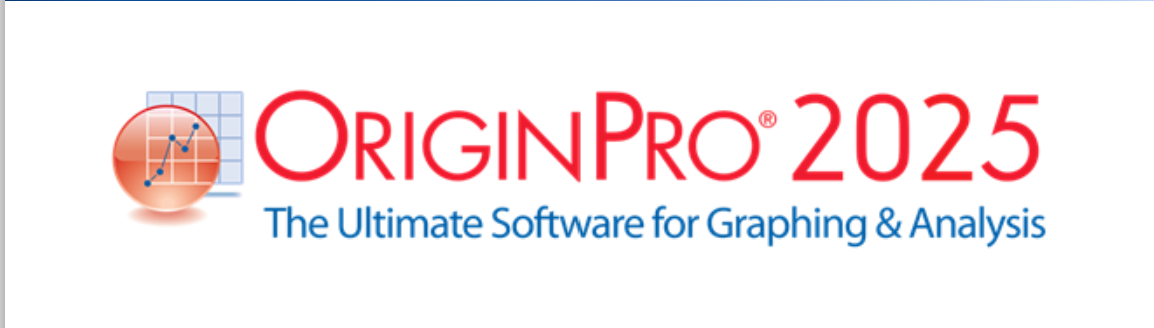
\includegraphics[scale=0.4]{origin.png}
    \caption{Origin}
\end{figure}
\par 这款软件可以在\href{https://software.ustc.edu.cn/zbh.php}{中国科学技术大学正版软件下载平台}进行下载
\subsubsection{Matlab}
Matlab是一款用于算法开发、数据可视化、数据分析以及数值计算的高级技术计算语言和交互式环境,可以进行矩阵运算,绘制图像等等工作,用途非常广泛,具体教程可见文档\href{https://github.com/kiri236/Guide-for-exchange-student-in-USTC/blob/main/docs/Matlab/Matlab%E7%94%A8%E4%BA%8EDSP%E5%85%A5%E9%97%A8%E6%8C%87%E5%8D%97_2024.docx}{Matlab用于DSP入门指南\_ 2024}或视频教程\href{https://www.bilibili.com/video/BV13kHVeMETZ/?spm_id_from=333.337.search-card.all.click&vd_source=1780915c6fb454598df0a5b955fb7565}{【MATLAB快速上手】45min搞定基础语法与使用技巧!}
\par 由于美国对中国科学技术大学进行了制裁,所以中国科学技术大学正版软件下载平台无法下载正版Matlab,请大家自行寻找学习版使用
\end{document}

